\documentclass[../DD0.tex]{subfiles}
\begin{document}

\section {User Interface Design}
\label{sec:ui}

  In this secrion we provide further details on the interface design of the Application. In the RASD document we provided a set of mockups that represent the overall feel of the Application screens. Here we will provide the navigation flow between the screens. The adopted syntax is \textbf{bold} for buttons, \textit{italics} for screens (referenced by figure number in the RASD document) and square brackets for conditional branches.

  \subsection{Screen flow graph for users}

    \begin{figure}[h!]
      \centering
      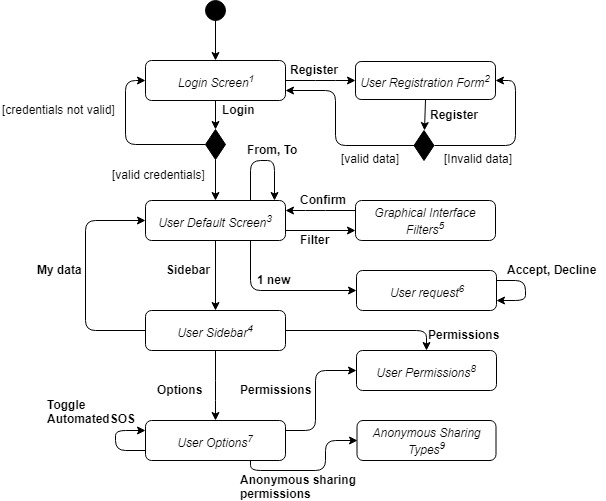
\includegraphics[width=\linewidth]{\fetchImg{util/GUIUser.jpg}}
      \caption{Flow of screens in the user application}
      \label{fig:flowuser}
    \end{figure}

    \subsection{Screen flow graph for third parties}

      \begin{figure}[h!]
        \centering
        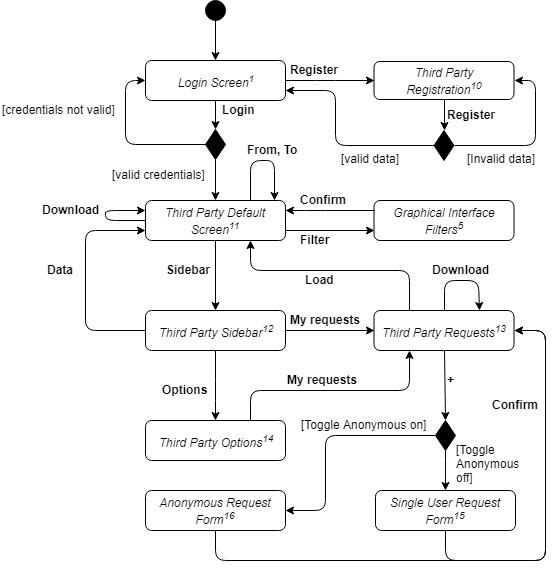
\includegraphics[width=\linewidth]{\fetchImg{util/GUIThirdParty.jpg}}
        \caption{Flow of screens in the third party application}
        \label{fig:flowthirdparty}
      \end{figure}

\end{document}
